

\documentclass{beamer}
 
\usepackage[utf8]{inputenc}
 \usetheme{Madrid}
 \usecolortheme{beaver}
 \usefonttheme{structuresmallcapsserif}
 \usepackage{listings}
%Information to be included in the title page:


\title[UI/UX] %optional
{User Interface/User eXperience}

\subtitle{An Overview in IoT}

\author[Dr. Joseph Kehoe] % (optional, for multiple authors)
{Joseph Kehoe\inst{1}}

\institute[IT Carlow] % (optional)
{
	\inst{1}%
	Department of Computing and Networking\\
	Institute of Technology Carlow
}

\date[ITC 2017] % (optional)
{CDD101, 2017}

\logo{
\includegraphics[height=1.5cm]{../../itcarlowlogo.png}}




 
 \AtBeginSection[]
 {
 	\begin{frame}
 		\frametitle{Table of Contents}
 		\tableofcontents[currentsection]
 	\end{frame}
 }
 
 
 
\begin{document}
 
\frame{\titlepage}
 
 
 
 \begin{frame}
 	\frametitle{Table of Contents}
 	\tableofcontents
 \end{frame}
 
 
 \section{Some Definitions}
 

  \begin{frame}
  	\frametitle{UI/UX}
  	\begin{description}
  		\item[UI] the means by which the user and a computer system interact, in particular the use of input devices and software;
  		\item[UX] the overall experience of a person using a product such as a website or computer application, especially in terms of how easy or pleasing it is to use.
  	\end{description}
  	
  	
  \end{frame}

  \begin{frame}
  	\frametitle{Early Interfaces}
  	\begin{itemize}
  		\item Input via Punch card
  		\item Output via Line Printer or (small) monochrome screen (or even LEDs)
  	\end{itemize}
  	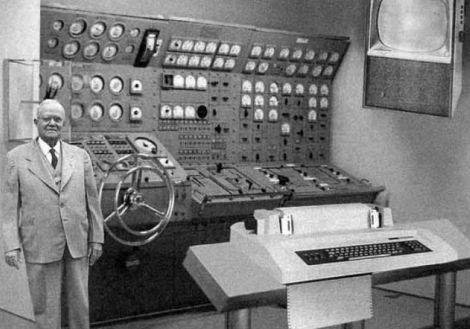
\includegraphics[height=4cm]{Old-Server.jpg}
  	
  \end{frame}
  
    \begin{frame}
    	\frametitle{CLI}
    	\begin{description}
    		\item[CLI] A command-line interface or command language interpreter (CLI), also known as command-line user interface, console user interface and character user interface (CUI), is a means of interacting with a computer program where the user (or client) issues commands to the program in the form of successive lines of text (command lines). 
    	\end{description}
    	A program which handles the interface is called a command language interpreter or shell. 
    	
    	Unix is the prime example today
    	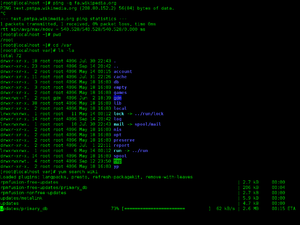
\includegraphics[height=3cm]{Bash.png}
    	
    \end{frame}
  
    \begin{frame}
    	\frametitle{GUI}
    	\begin{description}
    		\item[GUI] The graphical user interface, is a type of user interface that allows users to interact with electronic devices through graphical icons and visual indicators such as secondary notation, instead of text-based user interfaces, typed command labels or text navigation.
    	\end{description}
    	Windows, X Windows are best known examples (see also Smalltalk)
    	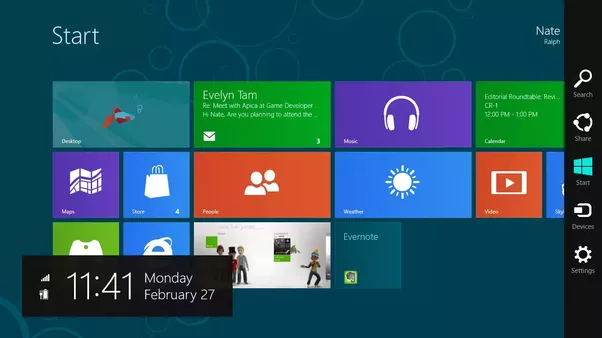
\includegraphics[height=3cm]{w10.png}
    	
    \end{frame}

     \begin{frame}
     	\frametitle{Mobile Device Interfaces}
     
    \begin{itemize}
    	\item  Output via Small Screen and Audio
    	\item Phone and Tablet
      
     \item Input via touch and voice
     \item Output via audio and screen
     
     \item Android, OS-X and Windows
    \end{itemize}
     
     	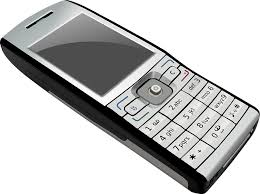
\includegraphics[height=4cm]{phone.jpeg}
     	
     \end{frame}

     \begin{frame}
     	\frametitle{Wearable Interfaces}
     	
     	\begin{itemize}
     		\item  May have no or tiny screen
     		\item May not have full (or easy) access
     		
     		\item Input via ?
     		
     		\item Output via ?
     		
     		\item Fitbit, Smartwatch, etc.
     	\end{itemize}
     	
     	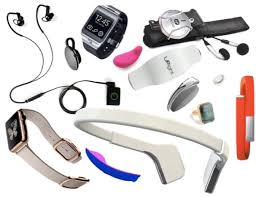
\includegraphics[height=4cm]{wearables.jpeg}
     	
     \end{frame}
      
           \begin{frame}
           	\frametitle{Alternate Interfaces}
           	
           	\begin{itemize}
           		\item  MMI
           		\item  NLP
           		\item  Video
           		\item  Gesture
           		\item Output via ?
           	\end{itemize}
           	
           	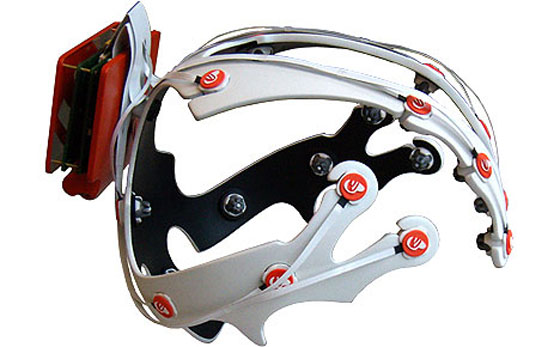
\includegraphics[height=4cm]{bci.jpg}
           	
           \end{frame}  
\end{document}

